%!Cau!%
\begin{ex}%[Đề tập huấn, Sở GD và ĐT - Quảng Trị, 2018]%[Nguyễn Văn Nay, 12EX10]%[1D3G2-2]
	Cho dãy số $\left(u_n\right)$ biết $u_1=1$ và $u_{n+1}=u_n+2n-1, \forall n \in \mathbb{N}^*$. Tính $u_{20}$.
	\choice
	{$u_{20}=364$}
	{\True $u_{20}=362$}
	{$u_{20}=361$}
	{$u_{20}=363$}
	\loigiai{
		Từ 	$u_{n+1}=u_n+2n-1, \forall n \in \mathbb{N}^* \Leftrightarrow u_{n+1}-u_n=2n-1, \forall n \in \mathbb{N}^*$.\\
		Do đó
		\begin{eqnarray*}
			&u_2-u_1&=1\\
			&u_3-u_2&=3\\
			&\vdots\\
			&u_n-u_{n-1}&=2(n-1)-1=2n-3
		\end{eqnarray*}
		Cộng vế theo vế ta có $u_n-u_1=1+3+\cdots+2n-3=(n-1)^2 \Rightarrow u_n=(n-1)^2+1$.\\
		Vậy $u_{20}=19^2+1=362$.
	}
\end{ex}%!Cau!%
\begin{ex}%[Thi thử, Lý Thái Tổ - Bắc Ninh, 2019]%[Nguyện Ngô, 12EX7]%[1D3G2-2]
Cho dãy số $(u_n)$ biết $\heva{&u_1=99\\&u_{n+1}=u_n-2n-1,\quad n\geq 1}$. Hỏi số $-861$ là số hạng thứ mấy?
\choice
{$35$}
{\True $31$}
{$21$}
{$34$}
\loigiai{
\begin{itemize}
\item $u_{n+1}=u_n-2n-1\Leftrightarrow u_{n+1}+(n+1)^2=u_n+n^2.$
\item Đặt $a_n=u_n+n^2$ ta có $a_{n+1}=a_n$ mà $a_1=u_1+1=100$ nên $a_n$ là dãy hằng, $a_n=100,\forall n\in\mathbb{N}$.
\item Vậy $u_n=100-n^2$, cho $-861=100-n^2\Leftrightarrow n=31$, vậy $-861$ là số hạng thứ $31$.
\end{itemize}
}
\end{ex}%!Cau!%
\begin{ex}%[Thi thử L1, Chuyên Lê Quý Đôn,Lai Châu, 2019]%[Nguyễn Tài Tuệ, dự án EX7]%[1D3G2-2]
	Cho $f_{0}(x)=x+|x-100|-|x+100|$ và với số tự nhiên $ n\ge 1 $, cho $f_{n}(x)=\left|f_{n-1}(x)\right|-1$. Có bao nhiêu giá trị của $ x $ để $f_{100}(x)=0$?
	\choice
	{$ 300 $}
	{\True $ 301 $}
	{$ 299 $}
	{$ 303 $}
	\loigiai{
		Ta có
		$f_n(x)=\left|f_{n-1}(x)\right|-1, \forall n \in \mathbb{N}^* \Rightarrow f_n(x) \ge -1,\, \forall n \in \mathbb{N}^*$. \\
		Nên $f_{100}(x)=0 \Leftrightarrow \left|f_{99}(x)\right|=1 \Leftrightarrow \left[\begin{aligned}
		&f_{99}(x)=1\\
		&f_{99}(x)=-1 .
		\end{aligned}\right. $
		\begin{itemize}
			\item $f_{99}(x)=1 \Leftrightarrow \left|f_{98}(x)\right|=2 \Leftrightarrow f_{98}(x)=2 \Leftrightarrow \left|f_{97}(x)\right|=3 \Leftrightarrow f_{97}(x)=3 \Leftrightarrow \cdots\Leftrightarrow f_1(x)=99 $\\
			$ \Leftrightarrow |f_0(x)|=100 \Leftrightarrow f_0(x)=\pm 100$.
			\item $f_{99}(x)=-1 \Leftrightarrow \left|f_{98}(x)\right|=0 \Leftrightarrow f_{98}(x)=0 \Leftrightarrow \left|f_{97}(x)\right|=1 \Leftrightarrow \left[\begin{aligned}
			&f_{97}(x)=1\\
			&f_{97}(x)=-1
			\end{aligned}\right. \Leftrightarrow \left[\begin{aligned}
			&f_{96}(x)=2\\
			&f_{96}(x)=0.\\
			\end{aligned}\right. $
			\item $f_{96}(x)=2 \Leftrightarrow f_{95}(x)=3 \Leftrightarrow f_{94}(x)=4 \Leftrightarrow \cdot \cdot \cdot \Leftrightarrow f_1(x)=97 \Leftrightarrow f_0(x)=\pm 98$.
			\item $f_{96}(x)=0 \Leftrightarrow f_{95}(x)=\pm 1$.
		\end{itemize}
		Tổng quát với mọi $k \in \mathbb{N}^*,k \leqslant 100$ ta có:
		\begin{itemize}
			\item $f_{2k+1}(x)=1 \Rightarrow f_0(x)=\pm (2k+2)$.
			\item $f_{2k+1}(x)=-1 \Rightarrow \left[\begin{aligned}
			&f_0(x)=\pm 2k\\
			&f_{2k-1}(x)=\pm 1.\\
			\end{aligned}\right. $
		\end{itemize}
		Do đó, $f_{100}(x)=0 \Leftrightarrow \left[\begin{aligned}
		&f_0(x)=\pm 100\\
		&f_0(x)=\pm 98\\
		& \cdots \\
		&f_0(x)=\pm 2\\
		&f_0(x)=0.\\
		\end{aligned}\right. $ \\
		Xét hàm số $f_0(x)=x+|x-100|-|x+100|$. \\
		Tập xác định $\mathbb{R}$. \\
		$f_0(x)=x+|x-100|-|x+100|=\heva{
			& x+200 & \text{ khi} x<-100\\
			&-x   & \text{ khi} -100 \le x \le 100\\
			& x-200 & \text{ khi} x>100.
		}. $ \\
		Bảng biến thiên của $f_0(x)$ \\
		\begin{center}
			\begin{tikzpicture}[scale=1]
			\tkzTabInit[nocadre=false,lgt=1.2,espcl=2.5,deltacl=0.6]
			{$x$/0.6,$f_0(x)$/2}{$-\infty$,$ -100 $,$0$,$100$,$+\infty$}
			%\tkzTabLine{,+,0,+,0,-,}
			\tkzTabVar{-/$-\infty$,+/$ 100 $ ,R/, -/$-100$ ,+/ $+\infty$}
			\tkzTabIma{2}{4}{3}{$0$}
			\end{tikzpicture}
		\end{center}
		Dựa vào bảng biến thiên ta có hai nhận xét\\
		+ Các phương trình $f_0(x)=0;f_0(x)=\pm 2;\ldots;f_0(x)=\pm 98$ mỗi phương trình có 3 nghiệm phân biệt (tổng cộng 99 phương trình).\\
		+ Các phương trình $f_0(x)=\pm 100$ mỗi phương trình có 2 nghiệm phân biệt.\\
		Vậy tổng số nghiệm là $99 \cdot 3+4=301$ nghiệm.}
\end{ex}